% ============================================================
%  Steam review analysis — project report
%  Build: tools\tectonic\tectonic.exe -X compile main.tex   (or upload the folder to Overleaf)
%  Title-page details (supervisor, date) are set just below.
% ============================================================
\documentclass[12pt,a4paper]{report}

% ---------- Title-page details: edit here ----------
\newcommand{\reporttitle}{STEAM REVIEW ANALYSIS: SENTIMENT CLASSIFICATION, ASPECT-BASED ANALYSIS AND GAME RECOMMENDATION}
\newcommand{\supervisorname}{Mr. Bui Van Hieu} % add the academic title (e.g. MSc.) if needed
\newcommand{\reportdate}{FPT University - November 2026}

% ---------- Encoding & Language ----------
\usepackage{iftex}
\ifXeTeX
  \usepackage{fontspec}
  \usepackage[protrusion=true]{microtype}
\else
  \usepackage[utf8]{inputenc}
  \usepackage[T1]{fontenc}
  \usepackage{lmodern}
  \usepackage[protrusion=true,expansion=true]{microtype}
\fi
\usepackage[english]{babel}

% ---------- Page Geometry & Spacing ----------
\usepackage{geometry}
\geometry{margin=1in}
\usepackage{setspace}
\onehalfspacing

% ---------- Figures, Tables, Math ----------
\usepackage{graphicx}
\graphicspath{{figures/}{Images/}}
\usepackage{booktabs}
\usepackage{tabularx}
\usepackage{longtable}
\usepackage{multirow}
\usepackage{float}
\usepackage{amsmath, amssymb}
\usepackage{array}
\usepackage{enumitem}
\usepackage{ragged2e}
\usepackage{algorithm}
\usepackage{algpseudocode}
\usepackage{xcolor}
\usepackage{caption}
\captionsetup{font=small,labelfont=bf}
\setlist{leftmargin=2em}
\renewcommand{\arraystretch}{1.15}
\newcolumntype{Y}{>{\RaggedRight\arraybackslash}X}
% let text and floats share pages instead of creating half-empty float pages
\renewcommand{\topfraction}{0.9}
\renewcommand{\bottomfraction}{0.8}
\renewcommand{\textfraction}{0.1}
\renewcommand{\floatpagefraction}{0.75}
\setcounter{topnumber}{3}
\setcounter{totalnumber}{4}
\setcounter{tocdepth}{1} % chapters and sections only: keeps the table of contents on one page

% ---------- Links ----------
\usepackage{hyperref}
\hypersetup{
    colorlinks=true,
    linkcolor=blue,
    citecolor=blue,
    urlcolor=blue,
    pdftitle={Steam Review Analysis: Sentiment Classification, Aspect-Based Analysis and Game Recommendation},
}

% ---------- Typography ----------
\usepackage[none]{hyphenat}
\sloppy

% ---------- Diagrams ----------
\usepackage{tikz}
\usetikzlibrary{positioning,arrows.meta,shapes.geometric,fit,calc}

% ---------- Frame of title page ----------
\newcommand{\pageframe}{%
  \begin{tikzpicture}[remember picture,overlay]
    \draw[line width=0.8pt]
      ([xshift=1cm,yshift=-1cm]current page.north west)
      rectangle
      ([xshift=-1cm,yshift=1cm]current page.south east);
  \end{tikzpicture}%
  \begin{tikzpicture}[remember picture,overlay]
    \draw[line width=0.8pt]
      ([xshift=1.1cm,yshift=-1.1cm]current page.north west)
      rectangle
      ([xshift=-1.1cm,yshift=1.1cm]current page.south east);
  \end{tikzpicture}%
}

\begin{document}

\begin{titlepage}
    \pageframe
    \begin{center}
        \vspace*{-1cm}

        % FPTU Logo
        
\includegraphics[width=0.6\linewidth]{Images/fpt_logo.png}

        \vspace*{0.25cm}

        \Large
        \textbf{\reporttitle}

        \vspace{0.2cm}
        \vfill
        \begin{table}[H]
        \large
        \centering
        \begin{tabular}{rl}
        Team members: & HE181627 - Le Sy Minh Quang \\
                      & HE176334 - Le Thanh Vinh \\
                      & HE181673 - Tran Vu Minh \\
                      &                           \\
        Supervisor:   & \supervisorname
        \end{tabular}
        \end{table}

        \vspace{0.25cm}
        \vfill
        \Large
        Bachelor of Artificial Intelligence\\
        \reportdate\\
    \end{center}
\end{titlepage}

\chapter*{Acknowledgements}

First and foremost, we would like to express our sincere gratitude to our instructor, Mr. Bui Van Hieu, for the guidance and feedback provided throughout this project. The suggestions received during the progress presentations, in particular the advice to group games by genre and publisher for recommendation and to explore keyword-based and transformer-based models, shaped a large part of the work reported here.

We are also thankful to the lecturers of FPT University, Hoa Lac campus, whose courses provided the foundations in machine learning and deep learning that this project builds on.

Finally, we thank our families and friends for their continuous support and encouragement during our studies.

\chapter*{Abstract}
\normalsize

User reviews on Steam combine free text with a single binary verdict (\textit{Recommended} or \textit{Not Recommended}). The verdict does not say which parts of a game players liked or disliked, and a noticeable share of reviews are jokes, sarcastic, or contradict their own verdict. This project builds a set of models on 10,000 English Steam reviews of 99 games to (1) classify review sentiment from text, (2) flag suspicious reviews whose content contradicts their verdict, (3) predict whether a review will receive helpful votes, (4) detect which aspects of a game a sentence talks about (graphics, audio, gameplay, story, performance, price, online, developer) and whether each aspect is praised or criticised, and (5) recommend games from the same genre or publisher group.

The baseline models are TensorFlow/Keras networks (embedding with pooling, BiLSTM, 1D CNN, TF-IDF with dense layers and an ensemble), compared against logistic regression baselines under two evaluation scenarios: known games and unseen games. The best Keras model reaches a ROC-AUC of 0.902/0.905, on par with TF-IDF logistic regression (0.903/0.906). Fine-tuning DistilBERT raises the ROC-AUC to 0.937/0.930, and the 95\% confidence interval of the gain excludes zero in both scenarios. For aspect-based analysis, about 4,600 sentences were labelled following written guidelines. Feeding keyword hints into DistilBERT and scoring each aspect with a pairwise model improves end-to-end F1 on a held-out test set from 0.451 to 0.622, and aspect polarity accuracy from 0.742 to 0.898. Sentences that praise one aspect and criticise another remain unsolved (accuracy about 0.55). The models are packaged into a local web application for review moderation and game recommendation. The aspect labels were drafted by a large language model following written guidelines and double-checked by the team.

\vspace{0.5cm}
\noindent\textbf{Keywords:} Sentiment Analysis; Aspect-Based Sentiment Analysis; Steam Reviews; TensorFlow; Keras; DistilBERT; Recommendation


\begin{singlespace}
\makeatletter
\renewcommand{\@makeschapterhead}[1]{{\parindent\z@\raggedright\normalfont\huge\bfseries #1\par\nobreak\vskip 20\p@}}
\makeatother
\tableofcontents
\listoffigures
\listoftables
\end{singlespace}
\clearpage

\chapter{Introduction}
\label{chap:introduction}

Steam is the largest digital distribution platform for PC games, and its user reviews are a main source of information for players deciding what to buy and for developers trying to understand how their game is received. Each review consists of a free-text body and a binary verdict: the reviewer either \textit{recommends} the game or does not. Steam aggregates these verdicts into summary labels such as ``Mostly Positive''.

The verdict is a coarse signal. It tells whether a player recommends a game, but not \textit{why}: one review may praise the graphics, criticise the crashes and still recommend the game. Moreover, many reviews are not serious evaluations at all: jokes, memes, sarcasm (``10/10 would never play again'') or texts that contradict the button the user pressed. Such reviews distort both the aggregated score and any analysis built on it.

This project studies what can be learned from the text of Steam reviews beyond the verdict. Using 10,000 English reviews of 99 popular games collected by the team through the Steam API, we build and evaluate models for review sentiment, suspicious review detection, helpfulness prediction, aspect-based sentiment analysis and game recommendation. As the course focuses on TensorFlow, the core models are implemented with TensorFlow/Keras; following the instructor's feedback, the project was then extended with keyword features and a pre-trained transformer (DistilBERT).

\section{Background and Motivation}

Sentiment classification of reviews is one of the most studied problems in natural language processing. Bag-of-words classifiers already perform well on movie reviews \cite{Pang2002}, recurrent \cite{Hochreiter1997} and convolutional \cite{Kim2014} networks learn their own text representations, and pre-trained transformers such as BERT \cite{Devlin2019} have become the standard approach when labelled data are limited.

Game reviews are a particular domain. In a study of the reviews of 6,224 Steam games, Lin \textit{et al.} \cite{Lin2019Steam} found that game reviews are relatively short, that the playtime before a review is a useful attribute specific to games, and that negative reviews carry most of the concrete complaints. Players use slang and inside jokes, mix praise and criticism, and often comment on patches and developers rather than on the game itself. This motivates two directions beyond plain sentiment classification: separating suspicious reviews from genuine ones, and identifying \textit{which aspects} of a game a review discusses. These tasks match practical needs: a platform can down-weight reviews that contradict their verdict or promote likely helpful reviews early, and a developer can see which aspects attract most criticism without reading hundreds of reviews. The instructor also suggested grouping games by genre and publisher to recommend similar games to players.

\section{Literature Review}

\textbf{Review-level sentiment.} Pang \textit{et al.} \cite{Pang2002} framed review sentiment as text classification with bag-of-words features and linear classifiers. Neural approaches replaced hand-crafted features with learned embeddings processed by LSTMs \cite{Hochreiter1997} or 1D convolutions \cite{Kim2014}. The transformer \cite{Vaswani2017} and large-scale pre-training \cite{Devlin2019} made it possible to fine-tune a general language model on a few thousand examples; DistilBERT \cite{Sanh2019} keeps most of BERT's accuracy with 40\% fewer parameters, which makes it practical on consumer GPUs.

\textbf{Aspect-based sentiment analysis (ABSA).} The SemEval-2014 shared task \cite{Pontiki2014} standardised ABSA into aspect category detection and aspect polarity on restaurant and laptop reviews. Sun \textit{et al.} \cite{SunABSA2019} showed that BERT handles ABSA well when the aspect is given to the model as an auxiliary sentence; our pairwise polarity model follows this idea.

\textbf{Sarcasm.} Riloff \textit{et al.} \cite{Riloff2013} describe sarcasm as a positive sentiment expressed about a negative situation, exactly the case where word-based classifiers fail and the text contradicts the reviewer's verdict.

\textbf{Research gap.} Public ABSA benchmarks cover restaurants or laptops; game reviews have other aspects (performance, monetisation, online community, developer support) and more humour and sarcasm.

\section{Problem Statement}

Given an English Steam review (with playtime and verdict where available), the project addresses five problems:
\begin{enumerate}
    \item \textbf{Sentiment classification:} predict whether the review is positive or negative from its content.
    \item \textbf{Suspicious review detection:} without labelled spam data, flag reviews whose content contradicts their verdict (sarcasm, trolling, misclicks) or that fail quality rules.
    \item \textbf{Helpfulness prediction:} estimate whether a review will receive a helpful vote, controlling for how long it has been online.
    \item \textbf{Aspect-based sentiment analysis:} detect which of eight aspects a sentence mentions and whether each is praised or criticised, then aggregate per game.
    \item \textbf{Game recommendation:} group games by genre and publisher and recommend games from the same group to users who liked a game.
\end{enumerate}

\section{Objectives and Contributions}

The objective is a reproducible pipeline that turns raw reviews into useful signals. Beyond solving the five tasks, the project documents the sampling biases of the data, compares five TensorFlow/Keras models with logistic regression baselines on known and unseen games, measures the gain of DistilBERT with confidence intervals and manual error analysis, evaluates the aspect pipeline on a test set labelled after the keywords were frozen, and packages the models into a local web application. The contribution is a careful comparison rather than a new architecture: which model helps, by how much, on which reviews, and where errors remain.

\section{Scope and Limitations}

The project covers English reviews of 99 games, binary sentiment and eight predefined aspects. The recommendation uses a small illustrative dataset with one review per user, so it is demonstrated but not quantitatively evaluated. Aspect labels were drafted by a large language model following written guidelines and double-checked by the team. Transformers run on Keras 3 with the PyTorch backend because recent TensorFlow releases do not support GPUs on native Windows. Chapter~\ref{chap:conclusion} discusses these limitations.

\section{Structure of the Report}

Chapter~\ref{chap:background} introduces the concepts and models used. Chapter~\ref{chap:data} describes the data, cleaning, exploration and labelling. Chapter~\ref{chap:methodology} presents the workflow, architectures and training setup. Chapter~\ref{chap:results} reports and analyses the results, and Chapter~\ref{chap:conclusion} concludes.

\chapter{Theoretical Background}
\label{chap:background}

This chapter introduces the concepts used in the project: text representation, the neural architectures for sentiment classification, transformers, aspect-based sentiment analysis and the evaluation metrics.

\section{Sentiment Classification and Text Representation}

Review sentiment is formulated as binary classification. Each review $x$ has a label $y \in \{0, 1\}$, where $y = 1$ means the reviewer recommended the game. A model outputs $\hat{p} = P(y = 1 \mid x)$ and is trained to minimise the binary cross-entropy
\begin{equation}
    \mathcal{L} = -\frac{1}{N}\sum_{i=1}^{N} \left[ y_i \log \hat{p}_i + (1 - y_i)\log(1 - \hat{p}_i) \right].
\end{equation}
The same loss is used for helpfulness ($y = 1$ if the review has a helpful vote) and, with one output per aspect, for aspect detection.

Classical models represent a text as a sparse vector of term weights. TF-IDF weights a term $t$ in document $d$ by its frequency and its rarity in the collection, $\text{tfidf}(t, d) = \text{tf}(t, d) \cdot \log (N / \text{df}(t))$, where $N$ is the number of documents and $\text{df}(t)$ the number of documents containing $t$. Word n-grams (``not good'') capture short-range negation and character n-grams tolerate spelling errors. Logistic regression then models $\hat{p} = \sigma(\mathbf{w}^\top \mathbf{x} + b)$ with the sigmoid $\sigma(z) = 1/(1 + e^{-z})$; with L2 regularisation it is a strong baseline for review sentiment \cite{Pang2002}.

\section{Neural Networks for Text}

A neural text model maps each token to a dense vector through a learned embedding matrix. Three ways of turning the sequence of vectors into one review representation are used in this project:
\begin{itemize}
    \item \textbf{Average pooling} takes the mean of the token vectors; it is fast but ignores word order.
    \item \textbf{LSTM} \cite{Hochreiter1997} reads the tokens in order and uses input, forget and output gates to decide what to keep in a memory cell, so it can capture negation and long-range context. A bidirectional LSTM runs one LSTM in each direction and concatenates their final states.
    \item \textbf{1D convolution} \cite{Kim2014} slides filters over the sequence to detect local phrases such as ``not worth'' wherever they occur, and keeps the strongest response of each filter by global max pooling.
\end{itemize}
To limit overfitting, dropout randomly zeroes activations during training and early stopping keeps the weights with the best validation loss.

\section{Transformers and DistilBERT}

The transformer \cite{Vaswani2017} replaces recurrence by self-attention. With queries $Q$, keys $K$ and values $V$,
\begin{equation}
    \text{Attention}(Q, K, V) = \text{softmax}\left(\frac{QK^\top}{\sqrt{d_k}}\right) V,
\end{equation}
so every token attends directly to every other token. BERT \cite{Devlin2019} pre-trains a deep transformer encoder on large text corpora by predicting masked words, and is then fine-tuned on a downstream task by adding a small output layer. Its input format \texttt{[CLS] text A [SEP] text B [SEP]} makes it natural to classify pairs of texts. DistilBERT \cite{Sanh2019} is a 6-layer version of BERT obtained by knowledge distillation; it is 40\% smaller and 60\% faster while keeping 97\% of BERT's language understanding, which makes it the largest model the team could fine-tune on a 4~GB GPU. Long inputs must be truncated, and keeping both the beginning and the end of a text works better than keeping only the beginning \cite{SunFinetune2019}.

\section{Aspect-Based Sentiment Analysis}

Aspect-based sentiment analysis (ABSA) decomposes an opinion into (aspect, polarity) pairs \cite{Pontiki2014}. With a fixed set of aspect categories it has two steps: \textbf{aspect detection}, a multi-label problem (a sentence may mention zero, one or several aspects), and \textbf{aspect polarity}, deciding for each detected aspect whether it is praised or criticised. A sentence-level model gives one polarity to the whole sentence and cannot handle ``great graphics but the servers are terrible''. Sun \textit{et al.} \cite{SunABSA2019} give the aspect to BERT as a second segment, \texttt{[CLS] aspect [SEP] sentence [SEP]}, so that the model scores that aspect only. We use this pairwise formulation for polarity, and a related idea for detection in which aspects proposed by keyword rules are given to the model as hints.

\section{Evaluation Metrics}

\textbf{ROC-AUC} is the main metric for binary tasks. It is the probability that a random positive example receives a higher score than a random negative one (0.5 is random guessing) and, unlike accuracy, it does not depend on a decision threshold. For aspect detection, precision $P = TP/(TP + FP)$, recall $R = TP/(TP + FN)$ and $F_1 = 2PR/(P + R)$ are computed by summing true positives, false positives and false negatives over all aspects (\textbf{micro F1}). In the end-to-end evaluation, a prediction is correct only if both the aspect and its polarity match the gold label.

\textbf{Confidence intervals.} Test sets contain from a few hundred to about two thousand examples, so differences between models must be checked against sampling noise. We use the paired bootstrap: the test examples are resampled with replacement 2,000 times, the difference between two models is computed on each resample, and the 2.5th and 97.5th percentiles form a 95\% confidence interval (CI). If the CI excludes zero, the difference is unlikely to be due to the particular test sample.

\chapter{Data Processing}
\label{chap:data}

This chapter describes the two datasets, how they were collected and cleaned, what the exploratory analysis revealed, and how additional LLM-assisted labels were created. Several findings here, in particular the sampling biases, determine which features the models may use.

\section{Dataset Description}

\subsection{Steam Reviews Dataset}

The main dataset was collected by the team through the public Steam review API between 21 and 28 September 2026. The target was the 50 most recent positive and 50 most recent negative reviews per game. The final file contains 10,000 reviews of 99 games written between December 2025 and September 2026: 95 games have exactly 100 reviews, while four deviate (Counter-Strike~2: 274, Dota~2: 126, Find The Needle Demo: 66, FiveM: 34), which is why the total is 10,000 rather than $99 \times 100$. Table~\ref{tab:columns} lists the fields; all reviews were identified as English by an automatic language detector.

\begin{table}[!htbp]
\centering
\caption{Fields of the Steam reviews dataset}
\label{tab:columns}
\begin{tabularx}{\textwidth}{lY}
\toprule
\textbf{Field} & \textbf{Description} \\
\midrule
\texttt{app\_id}, \texttt{game\_name} & Steam identifier and name of the game \\
\texttt{review\_id}, \texttt{review\_text} & Review identifier and raw review body \\
\texttt{voted\_up} & Recommendation verdict, used as a proxy label for review sentiment \\
\texttt{playtime\_forever\_hours} & Reviewer's total playtime at crawl time \\
\texttt{votes\_helpful} & Number of ``helpful'' votes received \\
\texttt{timestamp\_created} & Time the review was written \\
\bottomrule
\end{tabularx}
\end{table}

This collection procedure has two consequences that matter throughout the report:
\begin{itemize}
    \item The Recommended/Not Recommended ratio is balanced \textbf{by design} (about 50/50 for most games) and does not reflect each game's real reception, so per-game statistics can only be compared relatively.
    \item Negative reviews are rarer on Steam, so collecting 50 of them required going further back in time. The timestamp and the helpful votes (which accumulate over time) are therefore correlated with the label \textbf{because of the sampling}, not the content. Both are excluded from sentiment models; review age is used only as a control variable for helpfulness.
\end{itemize}

\subsection{Data Stream v2 (Recommendation Data)}

For the recommendation task suggested by the instructor, the data collection members of the team prepared a second file with 299 rows for 100 game entries, normally three reviewers per game from three tiers (users owning the most games, a mid-range user, users owning the fewest games); one entry (7 Days to Die) has no reviewer from the lowest tier, hence 299 rather than 300 rows. Each row contains games owned, reviews written, playtime, helpful and funny votes, the game's overall rating and a review excerpt in Vietnamese. The file shows signs of being simulated (regular text, exactly three reviewers per game, rounded numbers, eight games duplicated with identical rows), Steam IDs lost precision, and every user has a single review. The report therefore treats it as \textbf{illustrative data} for demonstrating recommendation, not as real reviews.

\section{Data Preprocessing and Cleaning}

\subsection{Cleaning the Steam Reviews}

The cleaning removes noise without discarding signals that carry sentiment (Table~\ref{tab:cleaning}). Emoji and censored words are kept because they carry sentiment: the \texttt{<censored>} token appears mostly in negative reviews. A rule flagging long runs of one repeated character was tried and dropped because it mostly caught legitimate texts such as ``-----'', ``!!!!'' or ``yesss''.

\begin{table}[!htbp]
\centering
\caption{Cleaning steps for the Steam reviews dataset}
\label{tab:cleaning}
\begin{tabularx}{\textwidth}{lY>{\RaggedRight\arraybackslash}p{3.4cm}}
\toprule
\textbf{Step} & \textbf{Method} & \textbf{Effect} \\
\midrule
De-duplication & Match texts after lower-casing and collapsing whitespace; keep the first copy; drop duplicate groups with conflicting labels & 29 removed (25 duplicates, 4 conflicts) \\
Markup removal & Remove Steam BBCode tags (keep their content) and URLs; de-duplicate again & 82 reviews modified \\
Normalisation & Replace the heart symbols of Steam's profanity filter by a \texttt{<censored>} token; keep emoji as separate tokens & No empty reviews \\
Quality flags & Truncated, repeated-word spam, too short, mixed language (flagged, not removed) & 20 reviews flagged \\
Name fixes & Normalise misspelled game names & 13 names \\
\bottomrule
\end{tabularx}
\end{table}

The final dataset has \textbf{9,971 reviews} (5,000 Recommended, 4,971 Not Recommended). The median review has 20 words and the mean 54.9 words, a strongly right-skewed distribution.

\subsection{Cleaning Data Stream v2}

Removing the duplicated games leaves \textbf{275 reviews of 92 games}. Reviewers received anonymous identifiers because the original Steam IDs were unusable, and the verdict was recovered from the wording of the rating field and checked against the text. Publishers were joined from an earlier team file (79 of 92 games) and completed manually; genres were assigned manually into 15 groups. The result has 69 publishers, 14 of them with at least two games. Survival (16 games) and builder/management (11) are the largest genres. In this illustrative data, 33\% of the reviews from users owning the fewest games are negative, against 6.5\% for the mid-range tier and none for the tier owning the most games.

\section{Exploratory Data Analysis and Feature Extraction}
\label{sec:eda}

The exploration looked for signals besides the text that relate to sentiment, and for artefacts of the data collection.
\begin{itemize}
    \item \textbf{The text is the main signal.} The strongest non-text feature has a mutual information with the label of only 0.044 (maximum 0.693). The class vocabularies differ clearly: \textit{fun, best, love} versus \textit{censored, boring, worst, crashes}.
    \item \textbf{Longer reviews lean negative} (Spearman $\rho = -0.26$), with the same sign in 96 of the 97 games that have at least 90 reviews.
    \item \textbf{Playtime has an inverted-U relation with sentiment} (Figure~\ref{fig:eda}): reviewers with less than two hours are positive in only 14\% of cases, against 57\% for 10--50 hours. Very short playtime often means refunds or games that do not start.
    \item \textbf{Explicit ``x/10'' scores} are strong but appear in only 4.4\% of reviews; question marks and censored words go with negative reviews.
    \item \textbf{Timestamp and helpful votes} correlate most with the label, but only because of the sampling.
\end{itemize}

\begin{figure}[!htbp]
    \centering
    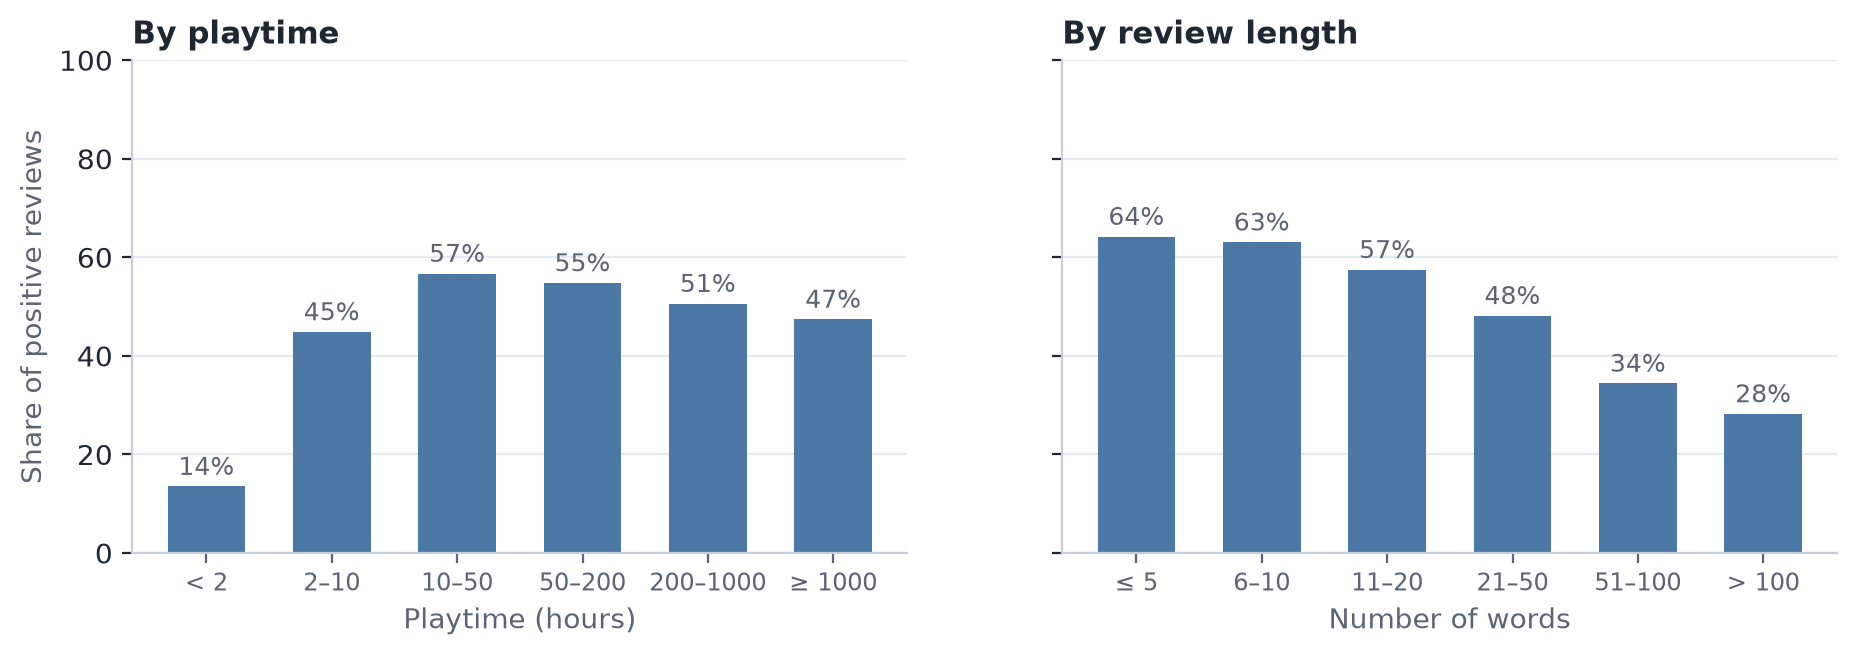
\includegraphics[width=0.9\textwidth]{fig02_eda.png}
    \caption{Share of positive reviews by playtime and by review length.}
    \label{fig:eda}
\end{figure}

From this analysis, ten \textbf{meta features} complement the text: the log word count, presence and value of an x/10 score, presence of a question mark, presence of a censored word, and playtime one-hot encoded into five bins ($<$2h, 2--10h, 10--50h, 50--200h, $\geq$200h). Playtime is binned because of its non-monotonic effect. Text features are learned by the models themselves.

\section{LLM-assisted Annotation}

The Steam verdict describes the whole review, so it cannot train or evaluate aspect-level models, nor tell whether an error comes from the model or from a misleading label. Additional labels were therefore drafted by a large language model (Claude) following written guidelines, without access to the Steam label, the game name or model predictions. The team then \textbf{reviewed every drafted label} (all 500 reviews and all 4,610 sentences) against the guidelines and corrected disagreements. No independent second annotation was made.

\textbf{Review labels.} 500 random reviews from test set A were labelled with a sentiment (217 negative, 187 positive, 71 unclear, 25 mixed) and a type (393 normal, 76 jokes or memes, 15 too short, 8 sarcastic, 8 off-topic). For reviews with a clear sentiment, the label agrees with the Steam verdict in 94.8\% of cases.

\textbf{Sentence labels.} Sentences were labelled with (aspect, polarity) pairs over eight aspects: graphics, audio, gameplay, story, performance/bugs, price/monetisation, online/community and developer; polarity is positive, negative, neutral or unclear. Generic sentences such as ``great game'' get no aspect. Table~\ref{tab:labelsets} lists the sets. Of the 4,610 labelled sentences, 4,461 are used: 97 keyword-selected sentences of an earlier dev split were dropped to keep dev random, and 52 training sentences from reviews that contribute dev sentences were dropped to avoid leakage. These sentence-level labels are independent of the Steam verdict. The keyword lists used as a baseline were written after reading Test 1, which favours them on that set, so Test 2 was labelled only after the keywords were frozen and is the main test set for aspect-level comparisons.

\begin{table}[!htbp]
\centering
\caption{LLM-assisted, team-reviewed labelled data}
\label{tab:labelsets}
\small
\begin{tabularx}{\textwidth}{lrYl}
\toprule
\textbf{Set} & \textbf{Size} & \textbf{Source} & \textbf{Purpose} \\
\midrule
Reviews & 500 & Random, test set A & Error analysis \\
Sentences, Test 1 & 500 & Random, test set A & Evaluation \\
Sentences, extra & 110 & Test set A, keyword-selected & Polarity examples \\
Sentences, Test 2 & 500 & Random, test set A, after keywords were frozen & Main evaluation \\
Sentences, dev & 438 & Random, outside test sets & Model selection \\
Sentences, train & 2,913 & Random, keyword-selected, conflicting & Training \\
\midrule
Sentences, total & 4,461 & 4,610 labelled, 149 unused & \\
\bottomrule
\end{tabularx}
\end{table}

\section{Data Splitting Strategy}
\label{sec:splits}

Two scenarios are used for review-level tasks (Table~\ref{tab:splits}). \textbf{Scenario A (known games)} is a stratified random 70/15/15 split. \textbf{Scenario B (unseen games)} holds out 20\% of the \textit{games} as the test set, which checks whether a model learns general ways of praising and complaining rather than game-specific words such as character or map names.

\begin{table}[!htbp]
\centering
\caption{Data splits for review-level tasks}
\label{tab:splits}
\begin{tabular}{llrrr}
\toprule
\textbf{Scenario} & \textbf{Set} & \textbf{Reviews} & \textbf{\% positive} & \textbf{Games} \\
\midrule
\multirow{3}{*}{A (known games)} & Train & 6,979 & 50.2 & 99 \\
 & Validation & 1,496 & 50.1 & 99 \\
 & Test & 1,496 & 50.1 & 99 \\
\midrule
\multirow{3}{*}{B (unseen games)} & Train & 6,813 & 50.0 & 79 \\
 & Validation & 1,203 & 50.0 & 79 \\
 & Test & 1,955 & 50.7 & 20 \\
\bottomrule
\end{tabular}
\end{table}

All splits use a fixed seed, so every model sees exactly the same data, and vocabularies, TF-IDF weights and scalers are fitted on the training set only. Sentence sets are split by review, and the code checks that no review contributes sentences to both training and dev or test data.

\chapter{Methodology}
\label{chap:methodology}

This chapter describes how the models are designed, trained and evaluated.

\section{Overall Workflow}

The project has three streams of work (Figure~\ref{fig:workflow}). The first builds review-level models with TensorFlow/Keras. The second, added after the instructor's feedback that the models were not deep enough, introduces LLM-assisted labels, keyword lists and DistilBERT for sentiment and aspect analysis. The third builds the game recommendation on Data Stream v2.

\begin{figure}[!htbp]
    \centering
    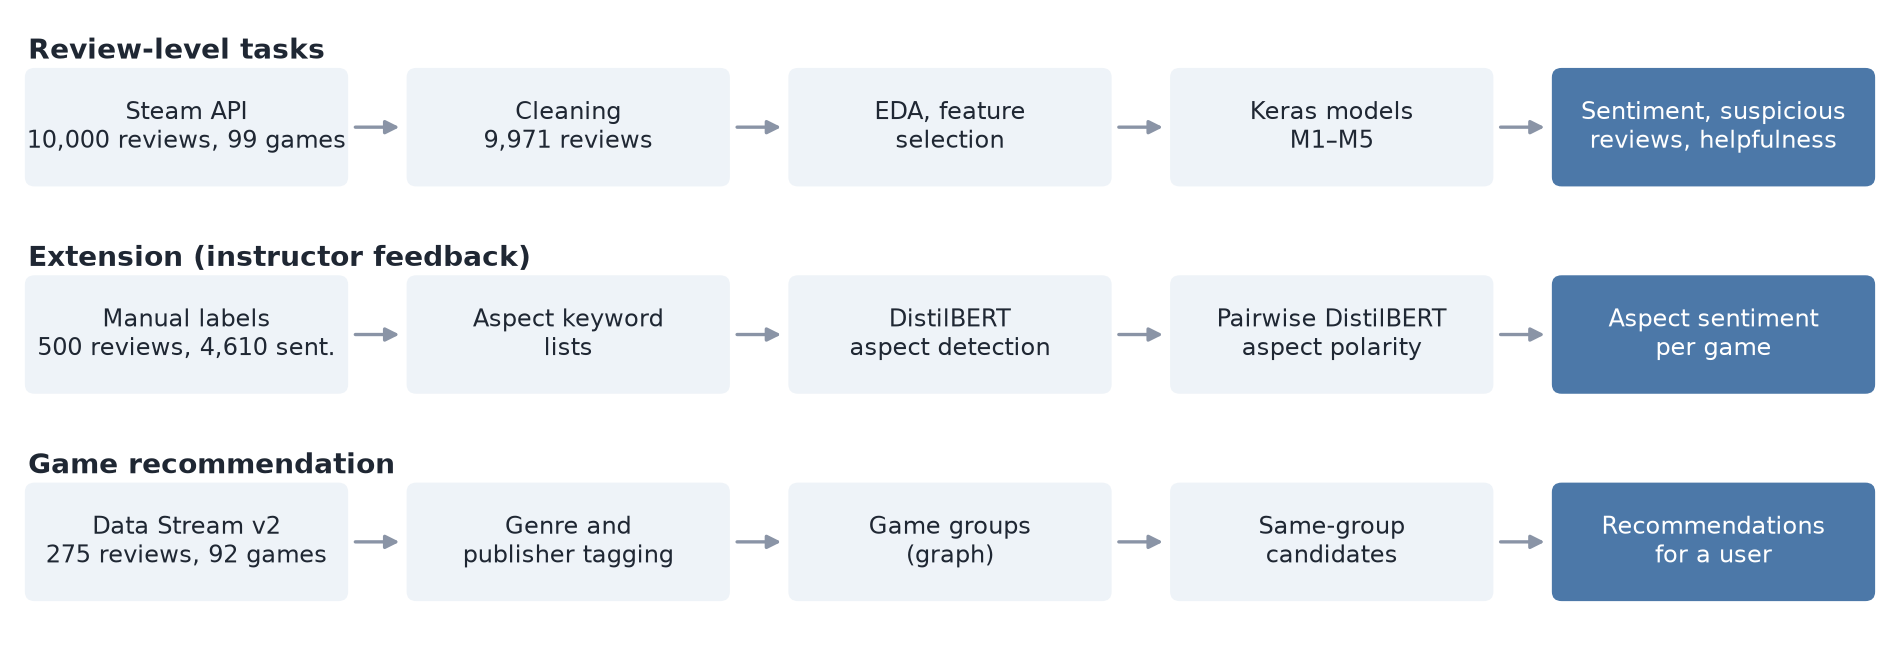
\includegraphics[width=\textwidth]{fig01_workflow.png}
    \caption{Overall workflow of the project.}
    \label{fig:workflow}
\end{figure}

In every experiment, hyperparameters, epochs and thresholds are chosen on the validation (dev) set and the test set is used only for reporting.

\section{Review-Level Models with TensorFlow/Keras}

\subsection{Baselines}

Three logistic regression (LR) baselines show how much information each input carries: \textbf{meta features only} (the ten features of Section~\ref{sec:eda}); \textbf{TF-IDF + LR} with word 1--2-grams (up to 50,000 features) and character 3--5-grams (up to 80,000 features); and \textbf{TF-IDF + meta + LR}. The regularisation strength $C$ is chosen from $\{0.25, \ldots, 8\}$ by validation ROC-AUC.

\subsection{Keras Architectures}

All Keras models share the two-branch structure of Figure~\ref{fig:kerasarch}, built with the functional API. In the \textbf{text branch}, a \texttt{TextVectorization} layer inside the model turns the raw string into token indices (256 tokens cover about 96\% of reviews in full) or into a TF-IDF vector. The \textbf{meta branch} normalises the ten meta features. The branches are concatenated and followed by a dense layer, dropout and a sigmoid output. Because vectorisation is part of the model, a saved \texttt{.keras} file accepts raw text.

\begin{figure}[!htbp]
\centering
\begin{tikzpicture}[
    node distance=0.35cm and 0.6cm,
    box/.style={rectangle, rounded corners=2pt, draw=black!60, fill=blue!8, minimum width=3.2cm, minimum height=0.65cm, align=center, font=\footnotesize},
    var/.style={box, fill=orange!15},
    io/.style={box, fill=gray!12, font=\footnotesize\bfseries},
    arr/.style={-{Stealth[length=2mm]}, thick, black!70}]
\node[io] (txt) {Review text (string)};
\node[box, below=of txt] (vec) {TextVectorization};
\node[var, below=of vec] (enc) {Text encoder M1--M4};
\node[io, right=0.7cm of txt] (meta) {10 meta features};
\node[box, below=of meta] (norm) {Normalization};
\node[box, below=of norm] (md) {Dense(16, ReLU)};
\node[box, below=0.8cm of $(enc)!0.5!(md)$] (cat) {Concatenate};
\node[box, below=of cat] (d32) {Dense(32) + Dropout(0.4)};
\node[io, below=of d32] (out) {Dense(1, sigmoid)};
\draw[arr] (txt) -- (vec); \draw[arr] (vec) -- (enc);
\draw[arr] (meta) -- (norm); \draw[arr] (norm) -- (md);
\draw[arr] (enc) |- (cat); \draw[arr] (md) |- (cat);
\draw[arr] (cat) -- (d32); \draw[arr] (d32) -- (out);
\node[font=\scriptsize, right=0.35cm of md, draw=black!30, rounded corners=2pt, inner sep=3pt, anchor=west] {%
\renewcommand{\arraystretch}{1.1}%
\begin{tabular}{@{}l@{\ }l@{}}
\textbf{M1:} & Embedding(64) $\rightarrow$ GlobalAvgPool \\
\textbf{M2:} & Embedding(64) $\rightarrow$ BiLSTM(64) \\
\textbf{M3:} & Embedding(64) $\rightarrow$ Conv1D(128, 5) $\rightarrow$ MaxPool \\
\textbf{M4:} & TF-IDF (30k) $\rightarrow$ Dropout(0.5) $\rightarrow$ Dense(32) \\
\textbf{M5:} & mean of the M2 and M4 outputs
\end{tabular}};
\end{tikzpicture}
\caption{Two-branch architecture shared by the Keras models.}
\label{fig:kerasarch}
\end{figure}

The models differ only in the text encoder (legend of Figure~\ref{fig:kerasarch}), following the text-classification labs of the course. M1 ignores word order, M2 captures order and negation, and M3 detects local phrases. M4 was added because M1--M3 did not beat the TF-IDF baseline: it brings n-gram TF-IDF features into a Keras network. M5 averages M2 and M4, which read the text differently (prediction correlation 0.85). Each model is trained separately for scenarios A and B.

\subsection{Suspicious Review Detection}

There are no labels for spam, trolling or sarcasm, so suspicious reviews are found from the disagreement between content and verdict, plus the quality rules (Algorithm~\ref{alg:suspicious}). M4 is trained in 5-fold cross-validation so that every review is scored by a model that has not seen it. The output is a ranked list of candidates for human review, not an automatic spam filter.

\begin{algorithm}[!htbp]
\caption{Suspicious review detection}
\label{alg:suspicious}
\begin{algorithmic}[1]
\For{each of 5 stratified folds $k$}
    \State Train M4 on the other folds; predict $p_i = P(\text{positive} \mid \text{text}_i)$ for reviews in fold $k$
\EndFor
\For{each review $i$ with Steam label $y_i$}
    \State $\text{mismatch}_i \gets (y_i = 0 \land p_i \geq 0.9) \lor (y_i = 1 \land p_i \leq 0.1)$
    \State $\text{suspicion}_i \gets |y_i - p_i|$ \Comment{0 = consistent, 1 = opposite}
    \State $\text{suspicious}_i \gets \text{mismatch}_i \lor \text{any quality flag}_i$
\EndFor
\State \textbf{return} suspicious reviews ranked by suspicion score
\end{algorithmic}
\end{algorithm}

The thresholds 0.9 and 0.1 keep only confident disagreements; reviews with $p$ close to 0.5 are reported separately as ``uncertain''.

\subsection{Helpfulness Prediction}

The target is whether a review had at least one helpful vote at crawl time (32.5\% of reviews), an observed label rather than a validated forecast of future votes; a binary target is used because 67.5\% of reviews have no vote. Older reviews have had more time to collect votes, so the log review age in days is added as a control variable. Inputs are the text, the meta features, review age and the sentiment label. Four models are compared: LR on age only, LR on meta features and age, TF-IDF + meta + age with LR, and Keras M4 on the same inputs with class weights for the minority class.

\section{Transformer Models}

\subsection{DistilBERT for Review Sentiment}

The pre-trained \texttt{distilbert-base-uncased} \cite{Sanh2019} is fine-tuned through Keras 3 and KerasHub. Inputs are limited to 128 tokens; for longer reviews the first and last parts are kept \cite{SunFinetune2019}, since reviewers often state their conclusion at the end. Token vectors are averaged (padding masked), followed by dropout 0.2 and a sigmoid output. The model uses the same splits as the Keras models, in both scenarios, with three seeds.

\subsection{Aspect Detection}

Aspect detection has eight sigmoid outputs, one per aspect, each with its own threshold chosen on dev. Five methods are compared: \textbf{keywords} (hand-written regular expressions per aspect, e.g. \texttt{crash|lag|fps} for performance), \textbf{TF-IDF + LR} (one balanced logistic regression per aspect), \textbf{DistilBERT} fine-tuned with eight outputs, the \textbf{union} of keywords and DistilBERT, and \textbf{keywords-in-input}. In the last method, the aspects found by the keywords are written before the sentence, \texttt{[CLS] graphics price [SEP] sentence [SEP]}, and DistilBERT decides whether to trust these hints, combining the precision of keywords with the transformer's ability to recognise paraphrases.
To measure the effect of labelled data, keywords-in-input is trained on 1,265, 1,995, 2,725 and 2,913 sentences, and plain DistilBERT on the smallest and largest sizes.

\subsection{Pairwise Aspect Polarity}

For each (sentence, aspect) pair the model receives \texttt{[CLS] aspect [SEP] sentence [SEP]}, with the aspect as one word (``graphics'', ``performance'', \ldots), and predicts whether that aspect is praised or criticised \cite{SunABSA2019}. A sentence with two aspects thus gets two independent predictions. Only pairs whose gold polarity is positive or negative are used, so this is a binary task. The encoder is initialised from a DistilBERT sentiment model fine-tuned on Steam labels, so it starts with knowledge of game-review sentiment. To target the hardest case, one training variant adds 188 sentences with a contrastive connective (``but'', ``however'') and at least two aspects. The baselines give every aspect of a sentence the sentence's polarity, predicted by M4 or by sentence-level DistilBERT.

\subsection{End-to-End Aspect Pipeline}

A review is split into sentences at sentence-ending punctuation and line breaks (keeping sentences of at least three words); each sentence goes through aspect detection, every detected aspect is scored by the pairwise model, and the pairs are aggregated per game (Figure~\ref{fig:absapipe}).

\begin{figure}[!htbp]
\centering
\begin{tikzpicture}[
    node distance=0.3cm,
    box/.style={rectangle, rounded corners=2pt, draw=black!60, fill=blue!8, minimum height=1.1cm, text width=1.9cm, align=center, font=\footnotesize},
    hl/.style={box, fill=orange!15, text width=2.5cm},
    arr/.style={-{Stealth[length=2mm]}, thick, black!70}]
\node[box] (r) {Review text};
\node[box, right=of r] (s) {Split into sentences};
\node[hl, right=of s] (d) {Aspect detection\\(keyword hints)};
\node[hl, right=of d] (p) {Pairwise polarity per aspect};
\node[box, right=of p] (g) {Aggregate per game};
\draw[arr] (r) -- (s); \draw[arr] (s) -- (d); \draw[arr] (d) -- (p); \draw[arr] (p) -- (g);
\end{tikzpicture}
\caption{End-to-end aspect-based sentiment pipeline.}
\label{fig:absapipe}
\end{figure}

\section{Game Recommendation}

Every user in Data Stream v2 wrote one review, so collaborative filtering, which needs users who rated several games, is not possible. A content-based method is used instead: games are compared by their attributes. Games, genres and publishers with at least two games form a graph in which each game is linked to its genre and publisher. For a user who liked game $g$, every other game $h$ is scored as
\begin{equation}
    \text{score}(h) = 2 \cdot \mathbf{1}[\text{genre}(h) = \text{genre}(g)] + \mathbf{1}[\text{publisher}(h) = \text{publisher}(g)],
\end{equation}
with ties broken by the overall positive rating of $h$. Genre has the larger weight because players usually look for the same type of game. If the user disliked $g$, highly rated games from other genres are suggested.

\section{Hyperparameters and Implementation}

Table~\ref{tab:hparams} lists the training settings. Transformers are scored on dev after each epoch and the best epoch is kept.

\begin{table}[!htbp]
\centering
\caption{Training configuration}
\label{tab:hparams}
\small
\begin{tabularx}{\textwidth}{lYY}
\toprule
\textbf{Setting} & \textbf{Keras models (M1--M4)} & \textbf{DistilBERT models} \\
\midrule
Optimizer & Adam & AdamW, weight decay 0.01, gradient clipping 1.0 \\
Learning rate & $10^{-3}$ ($3 \times 10^{-4}$ for M4) & $2 \times 10^{-5}$ ($3 \times 10^{-5}$ for aspect detection), 10\% warm-up, cosine decay \\
Batch size & 64 & 16 \\
Epochs & up to 15 (30 for M1), early stopping (patience 2) & 3 (sentiment), 6 (aspect detection), 5 (polarity) \\
Input length & 256 tokens, vocabulary 20,000 & 128 tokens, head + tail truncation \\
Regularisation & Dropout 0.4 (0.5 in M4), L2 $10^{-4}$ in M4 & Dropout 0.2 \\
Seeds & 1 & 3 (2 for some aspect variants) \\
\bottomrule
\end{tabularx}
\end{table}

The implementation uses Python 3.12 with pandas, NumPy, Matplotlib and \textbf{scikit-learn} (TF-IDF, LR baselines, splits, metrics). Keras models M1--M5 and the helpfulness model use \textbf{TensorFlow/Keras 2.20} on CPU (20--75 seconds per model). DistilBERT is fine-tuned with \textbf{Keras 3 and KerasHub on the PyTorch backend} on an NVIDIA GTX 1650 (4~GB), because recent TensorFlow versions do not support GPUs on native Windows (about 10 minutes per sentiment run, 2.5 hours for the final aspect experiment). A local \textbf{web application} (FastAPI and HTML/JavaScript) serves the Keras models of Tasks 1--3 and the recommendation (single-review analysis, batch moderation, data overview); the transformer checkpoints are not yet integrated into it.

\chapter{Results Analysis}
\label{chap:results}

This chapter reports the results of every task in the order of the problem statement, then discusses them. All numbers are measured on test data that were not used for training or model selection.

\section{Experimental Setup}

Review-level models are evaluated on the test sets of scenario A (1,496 reviews of known games) and scenario B (1,955 reviews of 20 unseen games) described in Section~\ref{sec:splits}, with ROC-AUC as the main metric and accuracy at a threshold of 0.5 as a secondary one. Aspect-level models are evaluated on the labelled sentence sets, with Test 2 as the main set. Transformer results are averaged over seeds, and a difference is considered reliable when its 95\% paired-bootstrap CI does not contain zero.

\section{Task 1: Review Sentiment Classification}

\begin{table}[!htbp]
\centering
\caption{Sentiment classification on the test sets of scenario A (known games) and B (unseen games)}
\label{tab:sentiment}
\begin{tabular}{lcccc}
\toprule
\multirow{2}{*}{\textbf{Model}} & \multicolumn{2}{c}{\textbf{Accuracy}} & \multicolumn{2}{c}{\textbf{ROC-AUC}} \\
\cmidrule(lr){2-3}\cmidrule(lr){4-5}
 & A & B & A & B \\
\midrule
Meta features only + LR & 0.661 & 0.657 & 0.716 & 0.711 \\
TF-IDF + LR & 0.818 & 0.827 & 0.903 & 0.906 \\
TF-IDF + meta + LR & 0.825 & 0.836 & 0.908 & 0.909 \\
\midrule
M1 Embedding + Pooling & 0.741 & 0.801 & 0.836 & 0.883 \\
M2 BiLSTM & 0.801 & 0.799 & 0.884 & 0.893 \\
M3 CNN 1D & 0.797 & 0.794 & 0.871 & 0.883 \\
M4 TF-IDF + Dense & 0.812 & 0.815 & 0.891 & 0.893 \\
M5 Ensemble (M2 + M4) & 0.824 & 0.826 & 0.902 & 0.905 \\
\midrule
DistilBERT (mean of 3 seeds) & $\approx$0.86 & $\approx$0.855 & \textbf{0.937} & \textbf{0.930} \\
\bottomrule
\end{tabular}
\end{table}

Table~\ref{tab:sentiment} leads to four observations:
\begin{itemize}
    \item \textbf{The text carries most of the information.} Meta features alone reach a ROC-AUC of about 0.71, TF-IDF + LR on the text 0.90; adding meta features to TF-IDF adds only 0.005.
    \item \textbf{Keras models trained from scratch do not beat TF-IDF + LR.} With fewer than 7,000 training reviews, M1--M3 start to overfit after 2--3 epochs. M4 is the best single Keras model, and the ensemble M5 matches the LR baseline (0.902 versus 0.903 in scenario A).
    \item \textbf{The models generalise to unseen games}: scores in scenario B are not lower than in scenario A, so the models learn general ways of praising and complaining rather than game-specific words.
    \item \textbf{DistilBERT is the best model}, with a ROC-AUC of 0.937 (A) and 0.930 (B). The 95\% CI of its gain over TF-IDF + LR is $[+0.026, +0.047]$ in scenario A and $[+0.017, +0.037]$ in scenario B, well above the variation between seeds (about 0.002).
\end{itemize}

\textbf{Error analysis.} M4 misses mild complaints more often than praise: on test set A, 25\% of negative reviews are classified as positive but only 13\% of positive reviews as negative, and accuracy drops from about 85\% for reviews longer than 50 words to 73\% for reviews of at most five words. The 500 manually labelled reviews show where the remaining difficulty lies (Table~\ref{tab:erroranalysis}). Both models are very accurate on clear reviews; jokes, mixed and unclear reviews are much harder. Reading the errors, DistilBERT reduces genuine model errors from 46 to 26, while errors caused by a Steam verdict that contradicts the text stay almost constant (13 and 14). No model can fix those, and they are exactly what Task 2 tries to find. Sarcasm such as ``Oh great, another update that breaks everything. Love it.'' is still read as positive by M4.

\begin{table}[!htbp]
\centering
\caption{ROC-AUC on the 500 manually labelled test reviews}
\label{tab:erroranalysis}
\begin{tabular}{lrcc}
\toprule
\textbf{Group of reviews} & \textbf{Reviews} & \textbf{M4} & \textbf{DistilBERT} \\
\midrule
All & 500 & 0.887 & 0.931 \\
Clear sentiment, normal reviews & 365 & 0.942 & 0.968 \\
Others (jokes, mixed, unclear, \ldots) & 135 & 0.672 & 0.758 \\
\bottomrule
\end{tabular}
\end{table}

\section{Task 2: Suspicious Review Detection}

The out-of-fold M4 predictions reach an accuracy of 0.82 and a ROC-AUC of 0.90, the same level as on the held-out test set, so they can serve as a measure of what the text says. Table~\ref{tab:suspicious} and Figure~\ref{fig:suspicious} summarise the result of Algorithm~\ref{alg:suspicious}.

\begin{table}[!htbp]
\centering
\caption{Suspicious reviews among the 9,971 cleaned reviews}
\label{tab:suspicious}
\begin{tabular}{lrr}
\toprule
\textbf{Criterion} & \textbf{Reviews} & \textbf{\%} \\
\midrule
Quality rules (any flag) & 20 & 0.20 \\
Content--verdict mismatch & 270 & 2.71 \\
\quad Negative text but recommended & 170 & 1.70 \\
\quad Positive text but not recommended & 100 & 1.00 \\
\midrule
\textbf{Suspicious (rules or mismatch)} & \textbf{290} & \textbf{2.91} \\
Uncertain model ($|p - 0.5| < 0.1$), reported separately & 1,078 & 10.81 \\
\bottomrule
\end{tabular}
\end{table}

\begin{figure}[!htbp]
    \centering
    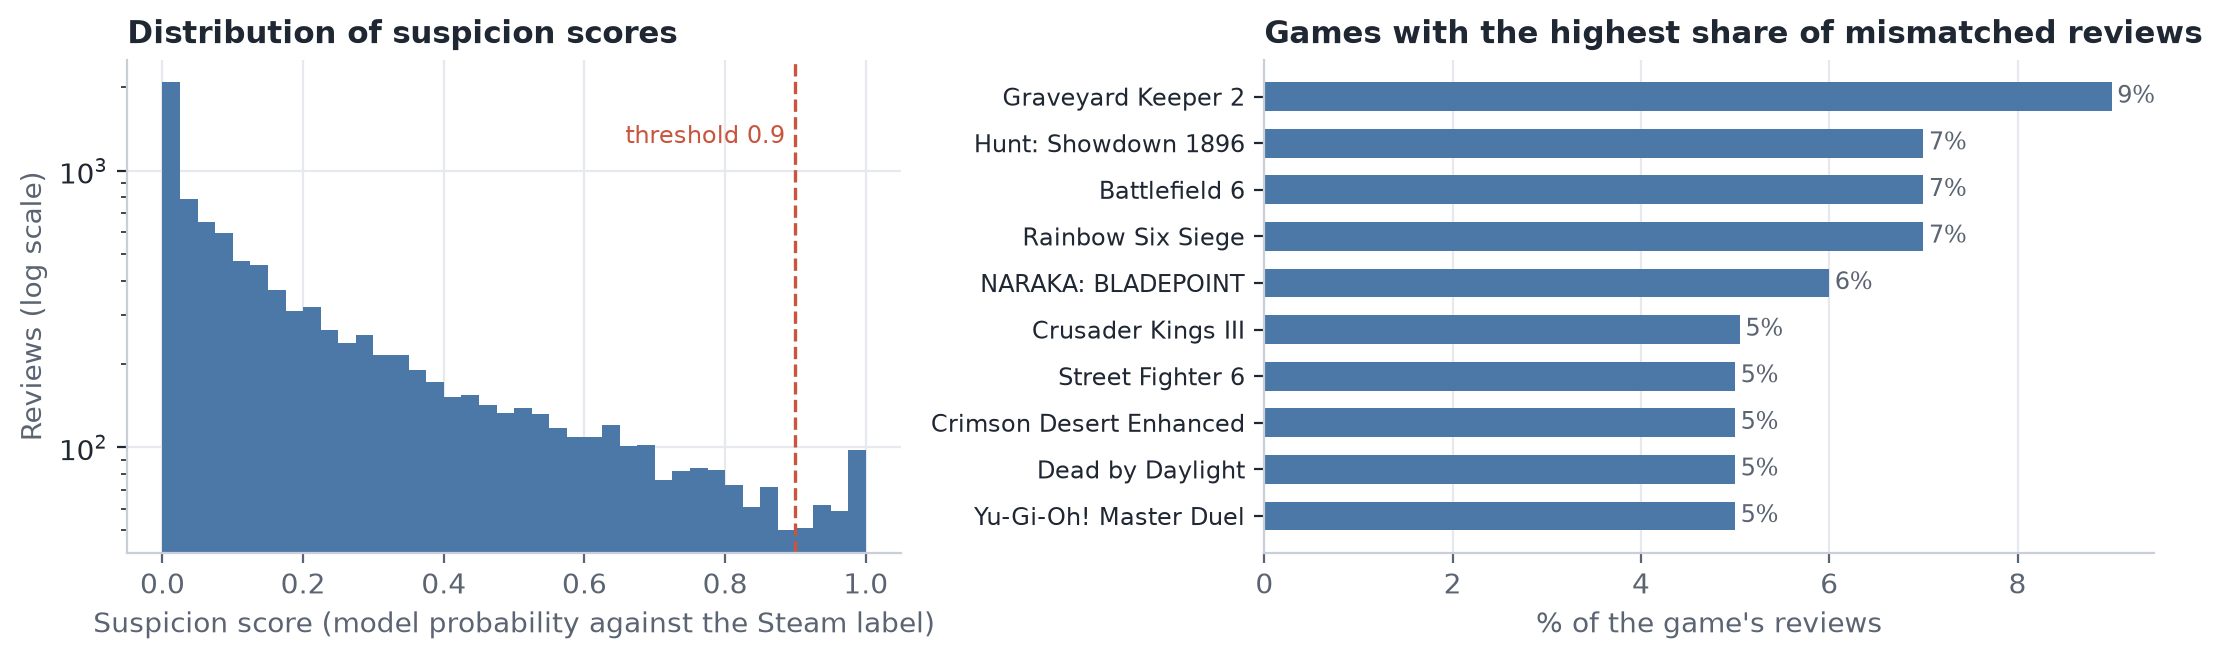
\includegraphics[width=0.95\textwidth]{fig13_suspicious.png}
    \caption{Distribution of suspicion scores (log scale) and games with the highest share of mismatched reviews.}
    \label{fig:suspicious}
\end{figure}

The quality rules catch only 20 reviews, so the cleaned data contain little obvious spam; the mismatch criterion is more informative. Reading the flagged reviews reveals three groups: \textbf{sarcasm and trolling} (``10/10 would never play again'', not recommended), \textbf{mixed reviews} that list strengths but conclude ``I can't recommend it'' or list bugs and still recommend, and \textbf{probable misclicks} with entirely positive text and a negative verdict. Several competitive online games are among those with the most mismatched reviews, but even for them the share stays below 10\%. Without ground-truth labels the precision of the flags cannot be computed, so the output is meant as a ranked list for human moderators rather than an automatic filter.

\section{Task 3: Helpfulness Prediction}

\begin{table}[!htbp]
\centering
\caption{Predicting whether a review receives at least one helpful vote (test set A)}
\label{tab:helpful}
\begin{tabular}{lccc}
\toprule
\textbf{Model} & \textbf{F1} & \textbf{ROC-AUC} & \textbf{PR-AUC} \\
\midrule
LR, review age only & 0.065 & 0.624 & 0.429 \\
LR, meta features + age & 0.515 & 0.771 & 0.601 \\
TF-IDF + meta + age, LR & 0.542 & \textbf{0.786} & \textbf{0.636} \\
Keras M4 + meta + age (class weights) & \textbf{0.611} & 0.761 & 0.605 \\
\bottomrule
\end{tabular}
\end{table}

Review age alone gives a ROC-AUC of 0.62, which confirms that it must be controlled for (Table~\ref{tab:helpful}). Meta features raise it to 0.77 and the text to 0.79, so content and length help beyond age. Keras M4 has a slightly lower ROC-AUC but the best F1 (0.61) thanks to class weighting. The strongest factor is the sentiment label: 51.9\% of negative reviews have a helpful vote against 13.2\% of positive ones, followed by review length. Because negative reviews in this dataset are also older, part of this effect comes from the sampling.

\section{Task 4: Aspect-Based Sentiment Analysis}

\subsection{Aspect Detection}

\begin{table}[!htbp]
\centering
\caption{Aspect detection (micro F1, mean over seeds). The variant selected on dev is in bold.}
\label{tab:aspectdet}
\begin{tabular}{lrccc}
\toprule
\textbf{Method} & \textbf{Train sentences} & \textbf{Dev} & \textbf{Test 2} & \textbf{Test 1} \\
\midrule
Keywords & 0 & 0.546 & 0.557 & 0.640 \\
TF-IDF + LR & 2,913 & 0.605 & 0.602 & 0.602 \\
DistilBERT & 1,265 & 0.655 & 0.606 & 0.635 \\
Keywords-in-input & 1,265 & 0.692 & 0.640 & 0.696 \\
Keywords-in-input & 1,995 & 0.708 & 0.665 & 0.714 \\
\textbf{Keywords-in-input} & \textbf{2,725} & \textbf{0.733} & \textbf{0.682} & \textbf{0.722} \\
Keywords-in-input & 2,913 & 0.731 & 0.692 & 0.731 \\
DistilBERT & 2,913 & 0.729 & 0.679 & 0.715 \\
Union of keywords and DistilBERT & 2,913 & 0.722 & 0.687 & 0.723 \\
\bottomrule
\end{tabular}
\end{table}

Table~\ref{tab:aspectdet} shows that:
\begin{itemize}
    \item \textbf{The transformer clearly beats keywords and TF-IDF.} On Test 2 the selected model is 0.125 above the keywords (CI $[0.085, 0.169]$) and 0.080 above TF-IDF + LR (CI $[0.040, 0.120]$).
    \item \textbf{Keyword hints help most when labels are scarce:} +0.033 over plain DistilBERT with 1,265 sentences, but only +0.003 with about 2,900 sentences, where the CI contains zero ($[-0.017, 0.024]$).
    \item \textbf{More labels help with diminishing returns}: +0.025, then +0.017 per additional 730 sentences.
    \item \textbf{Keywords alone have low recall} (precision 0.735, recall 0.448 on Test 2). Their higher score on Test 1 (0.640) reflects that they were written after reading that set, which justifies Test 2 as the main test set.
\end{itemize}
Per aspect, gameplay gains most over keywords (F1 0.47 to 0.71), because players describe gameplay in many ways that are hard to list. Online/community and developer remain harder (0.64 and 0.68), and audio (3 test sentences) and graphics (21) have too few examples for reliable conclusions.

\subsection{Aspect Polarity}

On the 765 (sentence, aspect) pairs with a positive or negative gold label, the pairwise model reaches an accuracy of 0.898, against 0.689 for always predicting ``negative'' (Table~\ref{tab:polarity}).

\begin{table}[!htbp]
\centering
\caption{Aspect polarity accuracy compared with whole-sentence models}
\label{tab:polarity}
\begin{tabular}{lccc}
\toprule
\textbf{Whole-sentence baseline} & \textbf{Accuracy} & \textbf{Pairwise gain} & \textbf{95\% CI} \\
\midrule
M4 & 0.742 & +0.156 & $[+0.125, +0.188]$ \\
DistilBERT & 0.835 & +0.063 & $[+0.042, +0.085]$ \\
\bottomrule
\end{tabular}
\end{table}

Two weaknesses remain. First, \textbf{sentences with conflicting aspects are not solved}: on the 55 pairs from sentences that praise one aspect and criticise another, all three models reach about 0.55 (ROC-AUC 0.58 for the pairwise model), and adding 188 such sentences to training changed nothing (0.552 versus 0.545). This was the case the pairwise formulation was meant to solve, so this objective was not met, although with 55 pairs the CI is wide ($[-0.145, +0.139]$ against M4). Second, \textbf{the model leans towards negative}: compared with M4, accuracy on negative pairs rises from 0.674 to 0.930, but on positive pairs it drops from 0.895 to 0.826.

\subsection{End-to-End Pipeline and Results per Game}

\begin{table}[!htbp]
\centering
\caption{End-to-end aspect sentiment pipeline (a pair is correct only if both aspect and polarity are correct)}
\label{tab:pipeline}
\begin{tabular}{lcccc}
\toprule
\multirow{2}{*}{\textbf{Pipeline}} & \multicolumn{3}{c}{\textbf{Test 2}} & \textbf{Test 1} \\
\cmidrule(lr){2-4}\cmidrule(lr){5-5}
 & P & R & F1 & F1 \\
\midrule
Keywords + M4 (first version) & 0.572 & 0.372 & 0.451 & 0.494 \\
Keywords + whole-sentence DistilBERT & 0.611 & 0.397 & 0.481 & 0.549 \\
Keywords + pairwise DistilBERT & 0.638 & 0.414 & 0.502 & 0.579 \\
\textbf{Keywords-in-input + pairwise DistilBERT} & 0.607 & \textbf{0.638} & \textbf{0.622} & \textbf{0.640} \\
\bottomrule
\end{tabular}
\end{table}

The end-to-end F1 rises from 0.451 to 0.622 (Table~\ref{tab:pipeline}), almost entirely through recall (0.372 to 0.638) while precision stays similar: the final pipeline finds many more aspect opinions without proportionally more mistakes. Both test sets rank the four pipelines in the same order.

Applied to all 33,025 sentences of the 99 games, the pipeline produced 24,223 (aspect, polarity) pairs; since some sentences were used in training, this is a description rather than an evaluation. Gameplay is by far the most discussed aspect (10,297 mentions). Players are most negative about performance and bugs (90.3\% of mentions) and developers (85.2\%), and least about graphics (31.0\%) and audio (43.7\%). Figure~\ref{fig:aspectgame} shows clear differences between games, the kind of summary a developer could use to prioritise fixes. The percentages should only be compared relatively, because of the 50/50 sampling per game, the longer negative reviews, the negative lean of the polarity model and the small number of sentences in some cells.

\begin{figure}[!htbp]
    \centering
    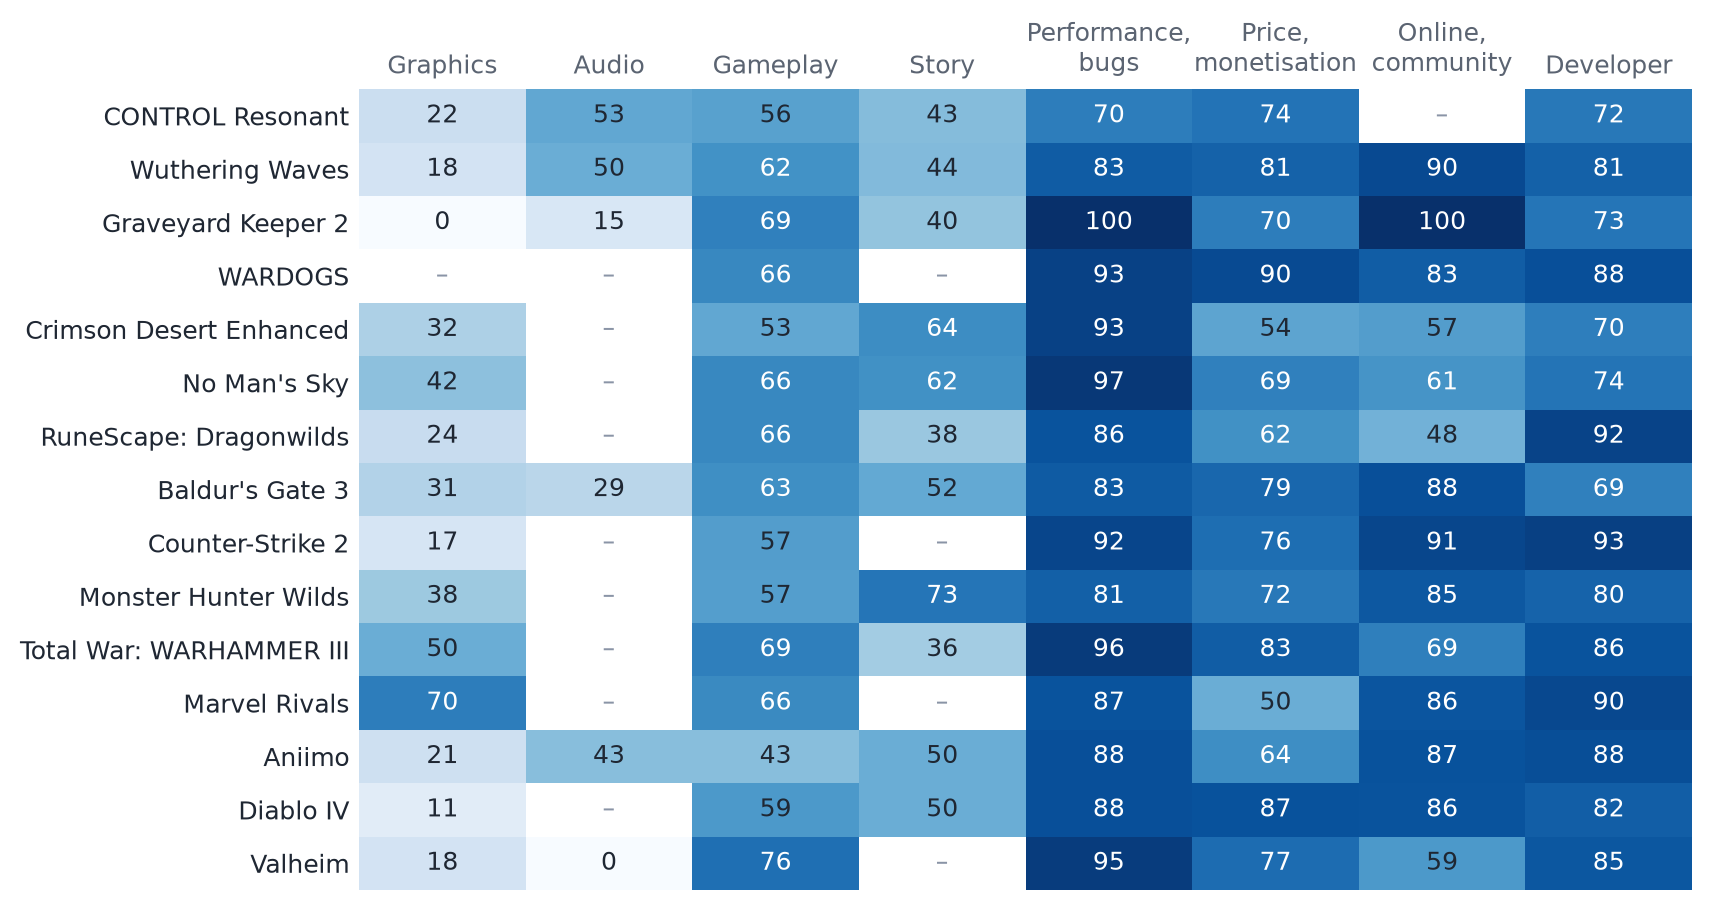
\includegraphics[width=0.75\textwidth]{fig10_aspect_by_game.png}
    \caption{Share of negative sentences (\%) per aspect for the 15 games with the most sentences; ``--'' marks fewer than 5 sentences.}
    \label{fig:aspectgame}
\end{figure}

\section{Task 5: Game Recommendation and Demo Application}

Figure~\ref{fig:appreco} shows the recommendation page of the demo application for a user who liked \textit{Stardew Valley}. Its genre is ``Life \& Job Sim'' and its publisher has no other game in the data, so all candidates share the genre and are ranked by their positive rating (Euro Truck Simulator 2, Slime Rancher and Dave the Diver at 97\%, then Slime Rancher 2 and Supermarket Simulator). The graph groups games around genre and publisher nodes, as suggested by the instructor. Because each user has a single review and there is no record of what users played next, the recommendations cannot be evaluated quantitatively; the result demonstrates the method. The other pages of the application apply the Task 1--3 models: for example, a clearly positive review submitted as ``Not recommended'' receives a positive probability of 99\% and is flagged as suspicious, and the batch page summarises all reviews of a game with the share of negative reviews by playtime and the most frequent words in negative reviews.

\begin{figure}[!htbp]
    \centering
    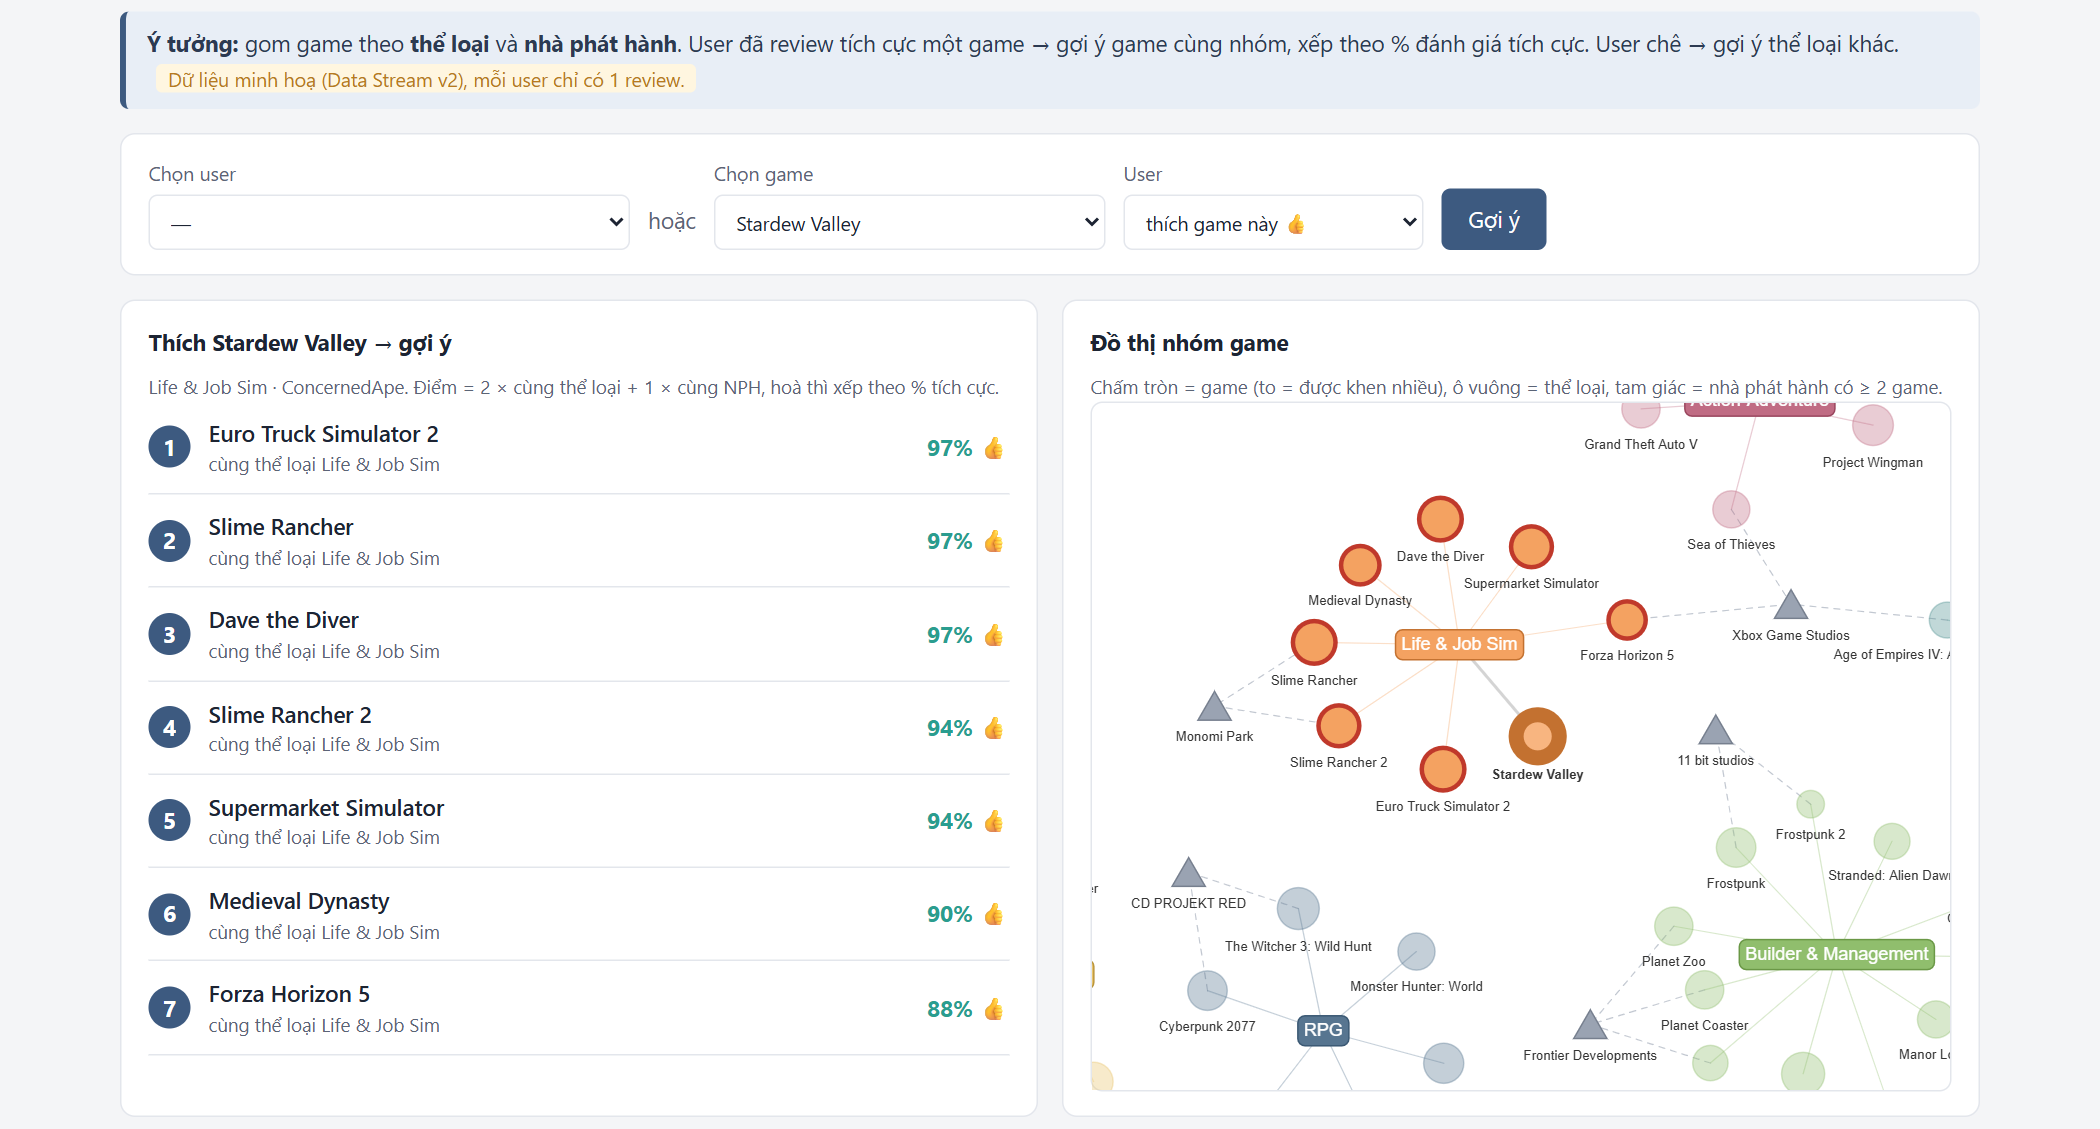
\includegraphics[width=0.88\textwidth]{app_reco.png}
    \caption{Recommendation page of the demo application (Vietnamese interface) for a user who liked Stardew Valley, with the genre/publisher graph.}
    \label{fig:appreco}
\end{figure}

\section{Discussion}

The results answer the instructor's question about deeper models with a nuanced picture. A pre-trained transformer gives a clear and statistically reliable improvement on every main metric (summarised in Table~\ref{tab:summary}); models trained from scratch on 7,000 reviews do not. Keywords are most useful as hints inside the transformer and when few labels are available. Where the transformer did not help, namely sentences with conflicting aspects, a likely cause is that each aspect's polarity depends on the clause structure of the sentence, which the model does not learn from a few hundred examples. Finally, part of the remaining sentiment errors comes from the verdicts rather than from the models, and these reviews are precisely what the suspicious review detector is designed to surface.

\chapter{Conclusion}
\label{chap:conclusion}

This project investigated what can be learned from the text of Steam reviews beyond the binary recommendation verdict.

\section{Summary of Achievements}

The data were cleaned into 9,971 reviews, and the exploration identified the text as the main signal and two sampling artefacts (timestamp and helpful votes) that would have leaked the label. Five Keras models trained from scratch reached a ROC-AUC of up to 0.902/0.905, on par with TF-IDF + LR and stable on unseen games. Out-of-fold predictions flagged 290 suspicious reviews (2.9\%), mostly sarcasm, mixed reviews and probable misclicks, and text features raised helpfulness prediction from a ROC-AUC of 0.62 (age only) to 0.79. Following the instructor's feedback, DistilBERT and keyword hints were added; Table~\ref{tab:summary} summarises the resulting gains. Applied to all 99 games, the aspect pipeline shows that players criticise performance and developers most and graphics least. A genre/publisher recommender and a local web application complete the project.

\begin{table}[!htbp]
\centering
\caption{Summary of the main results}
\label{tab:summary}
\small
\begin{tabularx}{\textwidth}{>{\RaggedRight\arraybackslash}p{4.3cm}Yll}
\toprule
\textbf{Task} & \textbf{Baseline} & \textbf{Best model} & \textbf{Result} \\
\midrule
Review sentiment, ROC-AUC (A / B) & TF-IDF + LR: 0.903 / 0.906 & DistilBERT & 0.937 / 0.930 \\
Aspect detection, micro F1 (Test 2) & Keywords: 0.557 & Keywords-in-input & 0.682 \\
Aspect polarity, accuracy & M4 whole sentence: 0.742 & Pairwise DistilBERT & 0.898 \\
End-to-end pipeline, F1 (Test 2) & Keywords + M4: 0.451 & Keywords-in-input + pairwise & 0.622 \\
\bottomrule
\end{tabularx}
\end{table}

The transformer improves every row of Table~\ref{tab:summary}; for the first three rows the 95\% CI of the gain over the baseline excludes zero (no CI was computed for the end-to-end pipeline). Keywords help most as input hints and when labels are scarce. The pairwise model raises polarity accuracy overall but does not solve sentences with conflicting aspects. The project therefore shows not only that a deeper model helps, but by how much, on which reviews, and where it does not.

\section{Limitations}

\begin{itemize}
    \item \textbf{Sampling.} The 50/50 sampling per game distorts sentiment ratios, helpful votes and timestamps; helpfulness results and per-game percentages should be read relatively.
    \item \textbf{Small groups.} Audio, graphics and conflicting-aspect sentences have few test examples; conflicting-aspect accuracy remains about 0.55 ($n = 55$).
    \item \textbf{Language and sarcasm.} Only English is handled, and mild sarcasm is often misclassified.
    \item \textbf{Recommendation data.} The recommendation uses illustrative data with one review per user and has no quantitative evaluation.
    \item \textbf{Environment.} Transformers run on Keras 3 with the PyTorch backend rather than TensorFlow, and are not yet integrated into the web application.
\end{itemize}

\section{Future Work}

\begin{enumerate}
    \item \textbf{Targeted labelling} of audio, graphics and conflicting-aspect sentences; the learning curve suggests a few more points for aspect detection.
    \item \textbf{Clause-level polarity:} split sentences at contrastive connectives before scoring, or use a model that attends explicitly to the aspect position.
    \item \textbf{Deploy the transformer models} in the web application so developers can see aspect summaries for their own reviews.
    \item \textbf{Better data:} reviews in natural proportions with real user identifiers, enabling realistic statistics, a fair helpfulness evaluation and collaborative filtering.
\end{enumerate}

In summary, simple baselines, TensorFlow/Keras models and a fine-tuned transformer together turn Steam reviews into useful signals: what players think of a game, which reviews to distrust, and which aspects need attention.


% ---------- References ----------
\bibliographystyle{IEEEtran}
\renewcommand{\bibname}{References}
\bibliography{references}

\end{document}
